% file : ProjectFebio.tikz
% author : Alicia Wang, Total SA
% date : May 2013
% 
% Structure of uncoupled solvers working independently before the coupling.
%------------------------------------------------------------------------------

\tikzstyle{selected} = [draw=red,fill=red!30]
\tikzstyle{optional} = [dashed,fill=gray!50]

\tikzstyle{term} = [draw=black, thick, rounded corners,%
                    text centered, text width = 30mm, minimum height = 10mm, anchor=center]

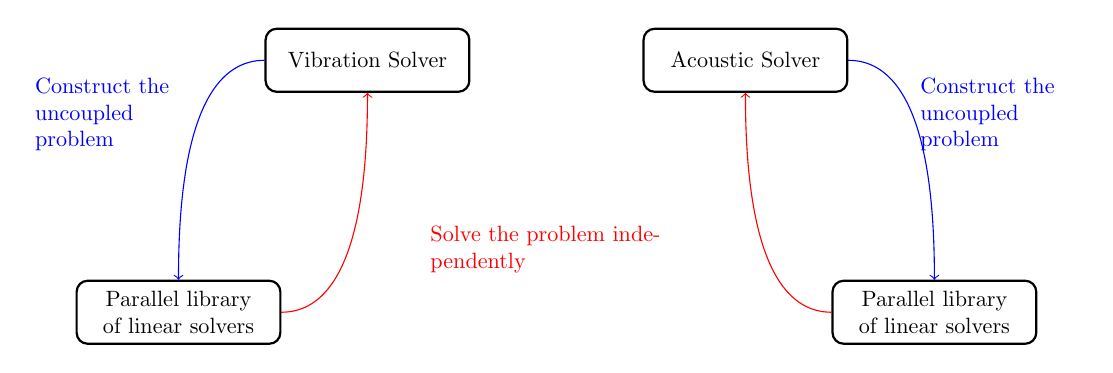
\begin{tikzpicture}[node distance = 30mm, every node/.style={scale=0.8}]

	
	\node (HSolidSolver) [term] {Vibration Solver};
	\node (cent) [term, draw = white, text width=10mm, right of = HSolidSolver] { };
	\node (HAcouSolver)  [term, right of = cent] {Acoustic Solver};
	\node (l1) [term, draw = white, text width=10mm, left of = HSolidSolver] { };
	\node (r1) [term, draw = white, text width=10mm, right of = HAcouSolver] { };
	
	\node (lib1) [term, below of = l1, node distance = 4cm] {Parallel library of linear solvers};
	\node (lib2) [term, below of = r1, node distance = 4cm] {Parallel library of linear solvers};
% 	\node (VACoupling)   [term, below of = cent, node distance = 60mm]  {Vibro-acoustic coupling Solver};
% 	\node		   (HPoroSolver)  [term, below of = VACoupling] {Harmonic Poro-elastic Solver};	
% 	\node		   (PoroVACoupling)[term, right of = HPoroSolver, fill=gray!30, node distance = 43mm] {Air/Poro-elastic/Solid coupling};
	
 	\draw[draw=blue,->] (HSolidSolver.west) .. controls +(left:1cm) and +(up:1cm) .. (lib1.north) node[pos=0.4, below, blue, text width=25mm, anchor = east] {Construct the uncoupled problem};
 	\draw[draw=blue,->] (HAcouSolver.east)  .. controls +(right:1cm) and +(up:1cm) .. (lib2.north) node[pos=0.4, below, blue, text width=25mm, anchor = west] {Construct the uncoupled problem};
 	
 	\draw[draw=red,->]  (lib1.east) .. controls +(right:1cm) and +(down:1cm) .. (HSolidSolver.south);
 	\draw[draw=red,->]  (lib2.west) .. controls +(left:1cm) and +(down:1cm) .. (HAcouSolver.south);
 	
 	\node (centNote) [red, draw = white, text width=40mm, below of = cent] {Solve the problem independently};
 	
%  	\draw[draw=green,->] (HSolidSolver.south) -- (VACoupling.north) node[pos=0.5, green, sloped, above] {\small{Construct the coupling interface}};
%  	\draw[draw=green,->] (HAcouSolver.south)  -- (VACoupling.north);
%  	
%  	\draw[draw=red,->] (VACoupling.west) .. controls +(left:1cm) and +(down:1cm) .. (lib1.south);
%  	\draw[draw=red,->] (VACoupling.east) .. controls +(right:1cm) and +(down:1cm) .. (lib2.south);
%  	
%  	\node (VAnote) [red, below of = VACoupling, node distance = 12mm] {\small{Pilote the two libraries for the global iterative methods}};
 	
 	
% 	\draw[draw=blue, dashed,->] (VACoupling.south)--(HPoroSolver.north);
% 	\draw[draw=blue,->] (HPoroSolver.east)--(PoroVACoupling.west);
% 	
% 	\node (algo) [term, draw=red, above of = PoroVACoupling, node distance = 30mm] {Adjustment of algorithms};
% 	
% 	\draw[draw=red,<->,opacity=.5] (algo.west) to[bend right] (VACoupling.north);
% 	\draw[draw=red,<->,opacity=.5] (algo.south)--(PoroVACoupling.north);
% 	
% 	
% 	
% 	\draw[draw=green,->,opacity=.6] (HAcouSolver.south west) to[bend right] (lib.north west);
% 	\draw[draw=green,->,opacity=.6] (HSolidSolver.west) to[bend right] (lib.west);
% 	\draw[draw=green,->,opacity=.6] (HPoroSolver.south) -- (lib.north);
% 	
% 	\node (link) [green!70,xshift=-4cm,above of=lib, node distance=6mm] {L I N K E D \hspace*{2mm} T O};
\end{tikzpicture}